
%\section{Configurar smartphone en modo de Depuracion}

\begin{frame}
\frametitle{Configurar telefono inteligente en modo de desarrollador (0)}  
\begin{itemize}
\item Es necesario buscar en las opciones de configuraci\'on, en el apartado acerca del telefono ubicar el n\'umero de compilaci\'on 
\item Dar 5 taps (toques) sobre el n\'umero compilaci\'on. Debera aparecer un mensaje que diga que estas a X taps de ser un desarrollador 
\item Lo anterior habilita un nuevo men\'u en el apartado sistema dentro de opciones de configuraci\'on con t\'itulo ``opciones para desarrolladores'' 
\item Debe habilitarse tanto ``opciones para desarrolladores'' como la opci\'on ``depuraci\'on USB''
\end{itemize}

\end{frame}



\begin{frame}
\frametitle{Configurar telefono inteligente en modo de desarrollador (1)}  
\begin{columns}
\column{0.25\linewidth}
\begin{center}
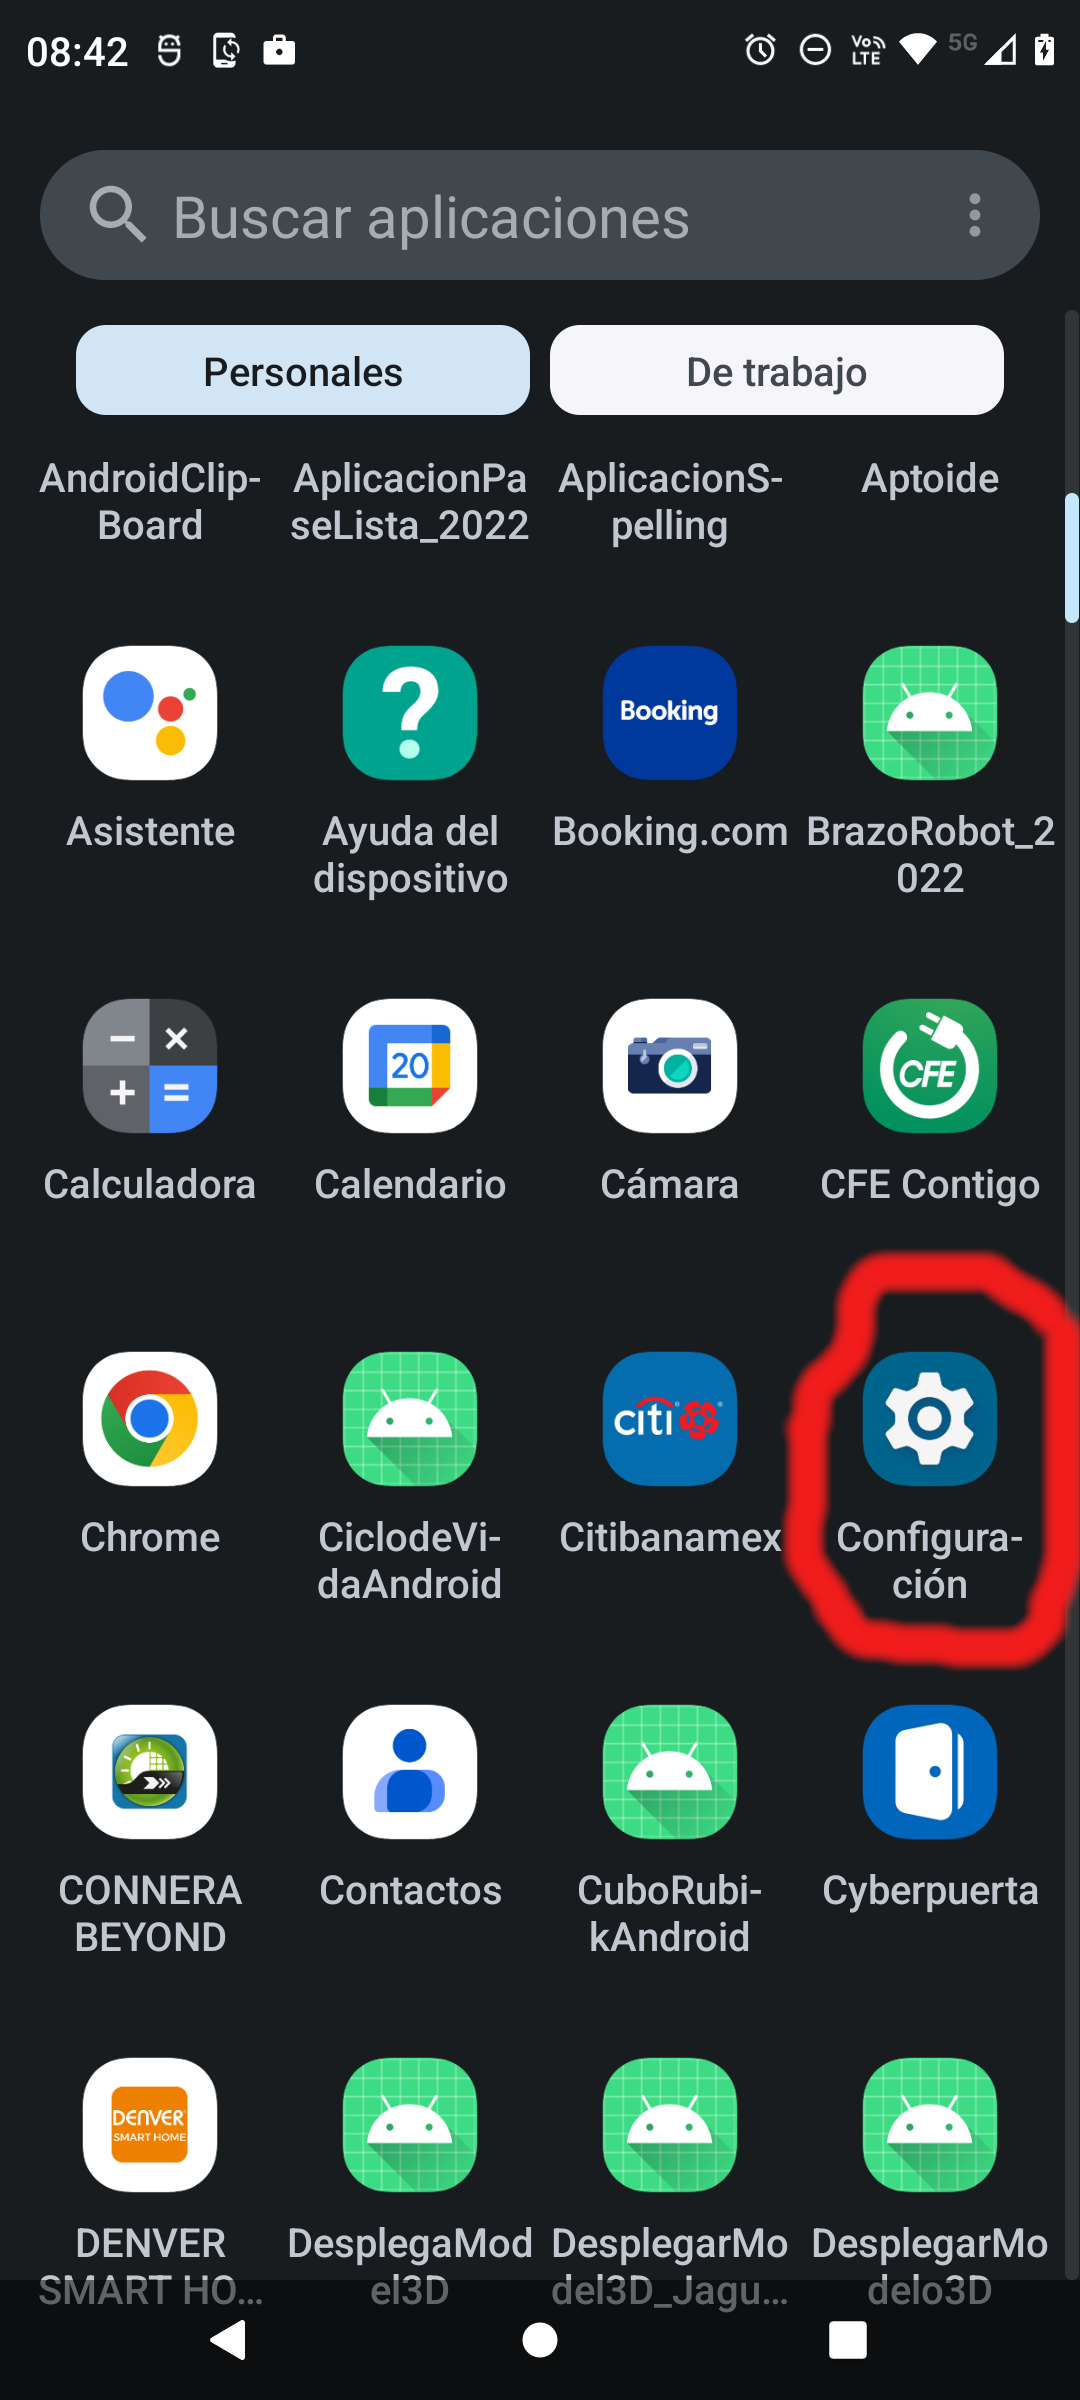
\includegraphics[width=0.95\linewidth]{01_Configurar/ModoDesarrollador1.png}    
\end{center}
\column{0.25\linewidth}
\begin{center}
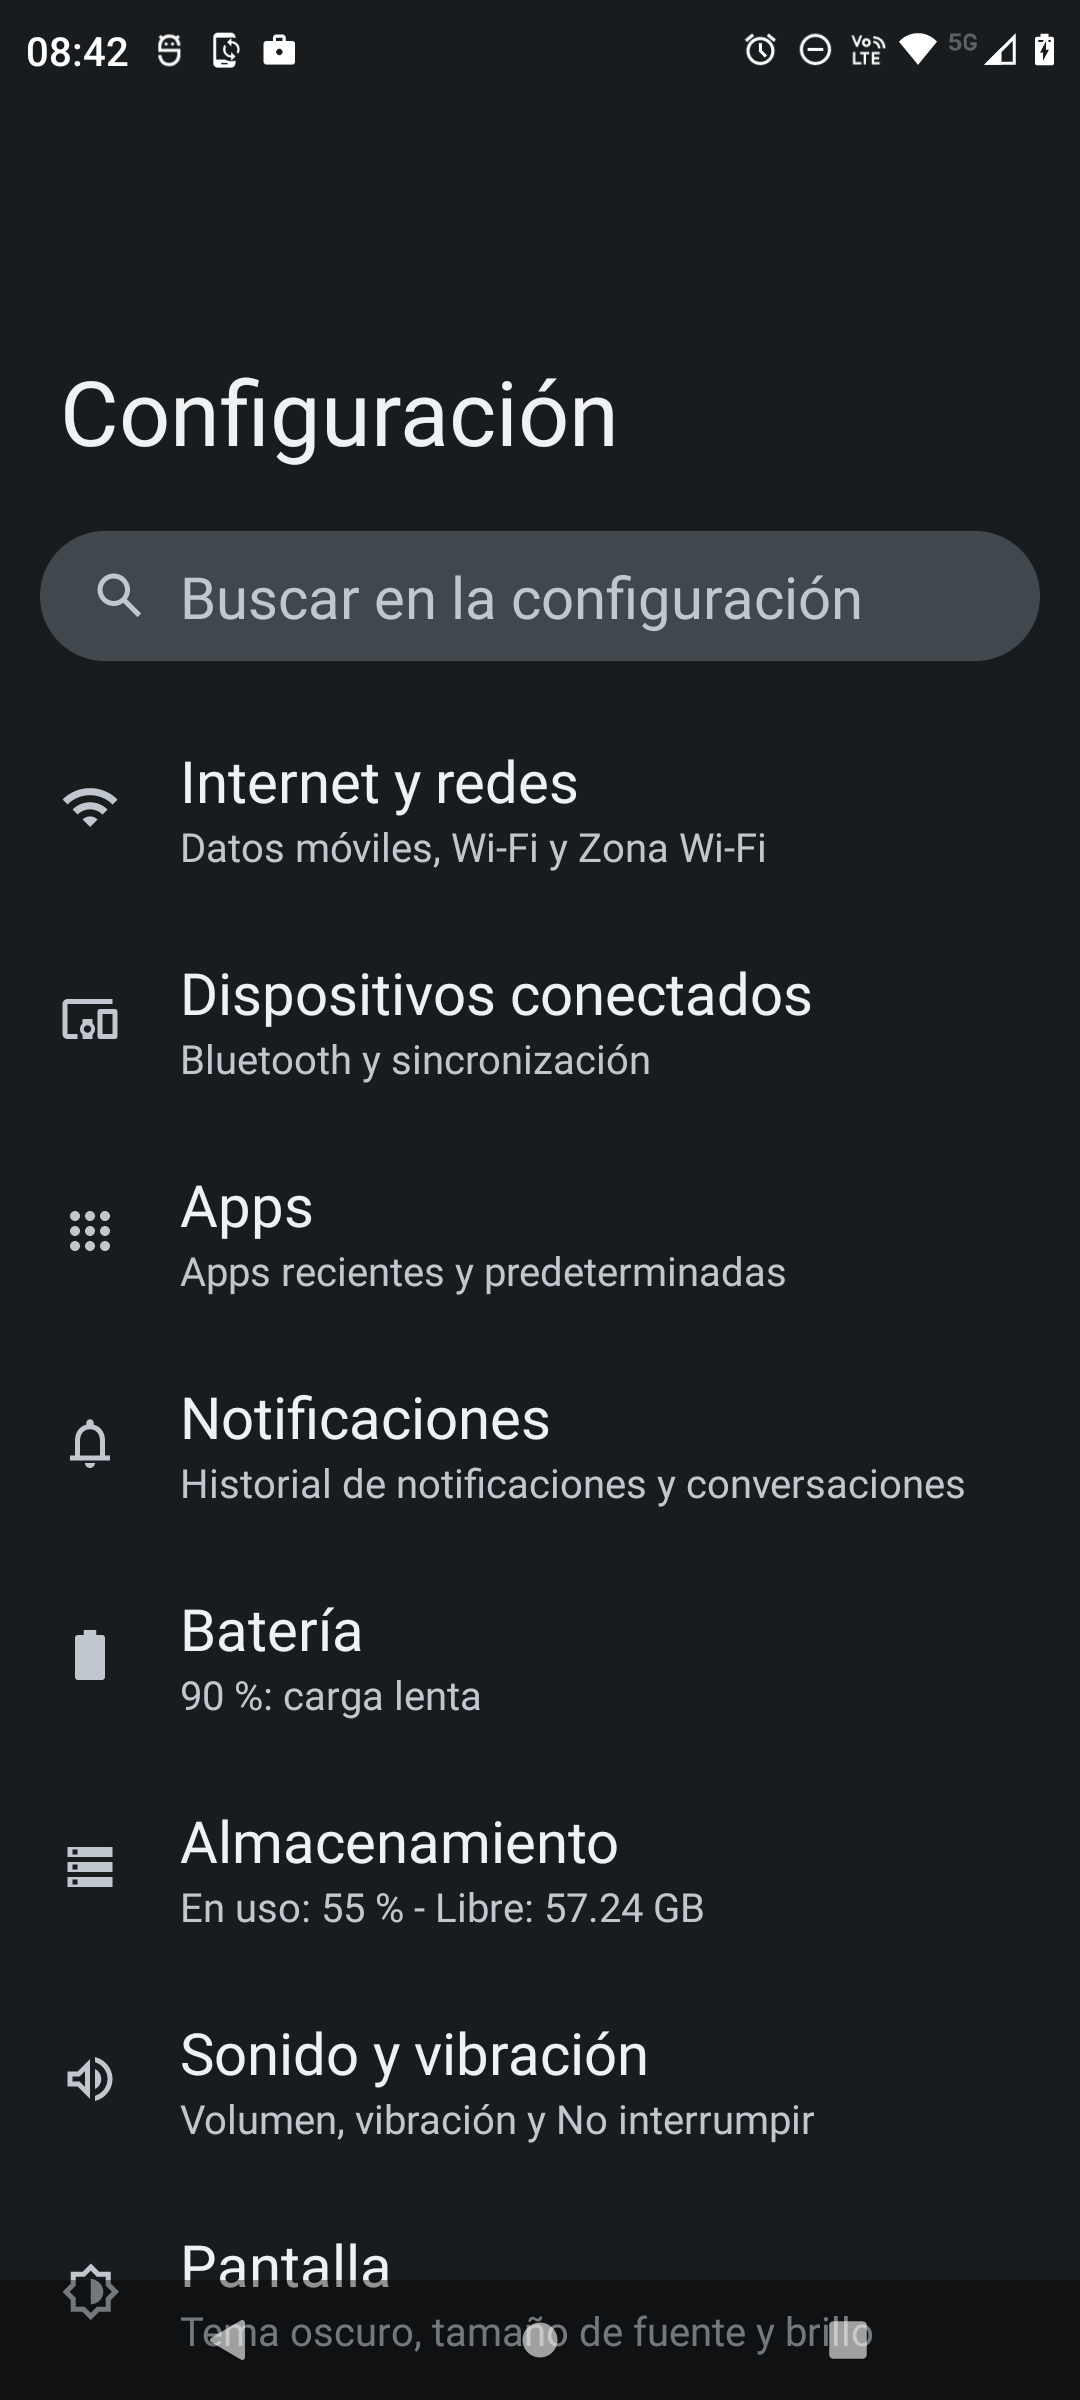
\includegraphics[width=0.95\linewidth]{01_Configurar/ModoDesarrollador2.png}    
\end{center}
\column{0.25\linewidth}
\begin{center}
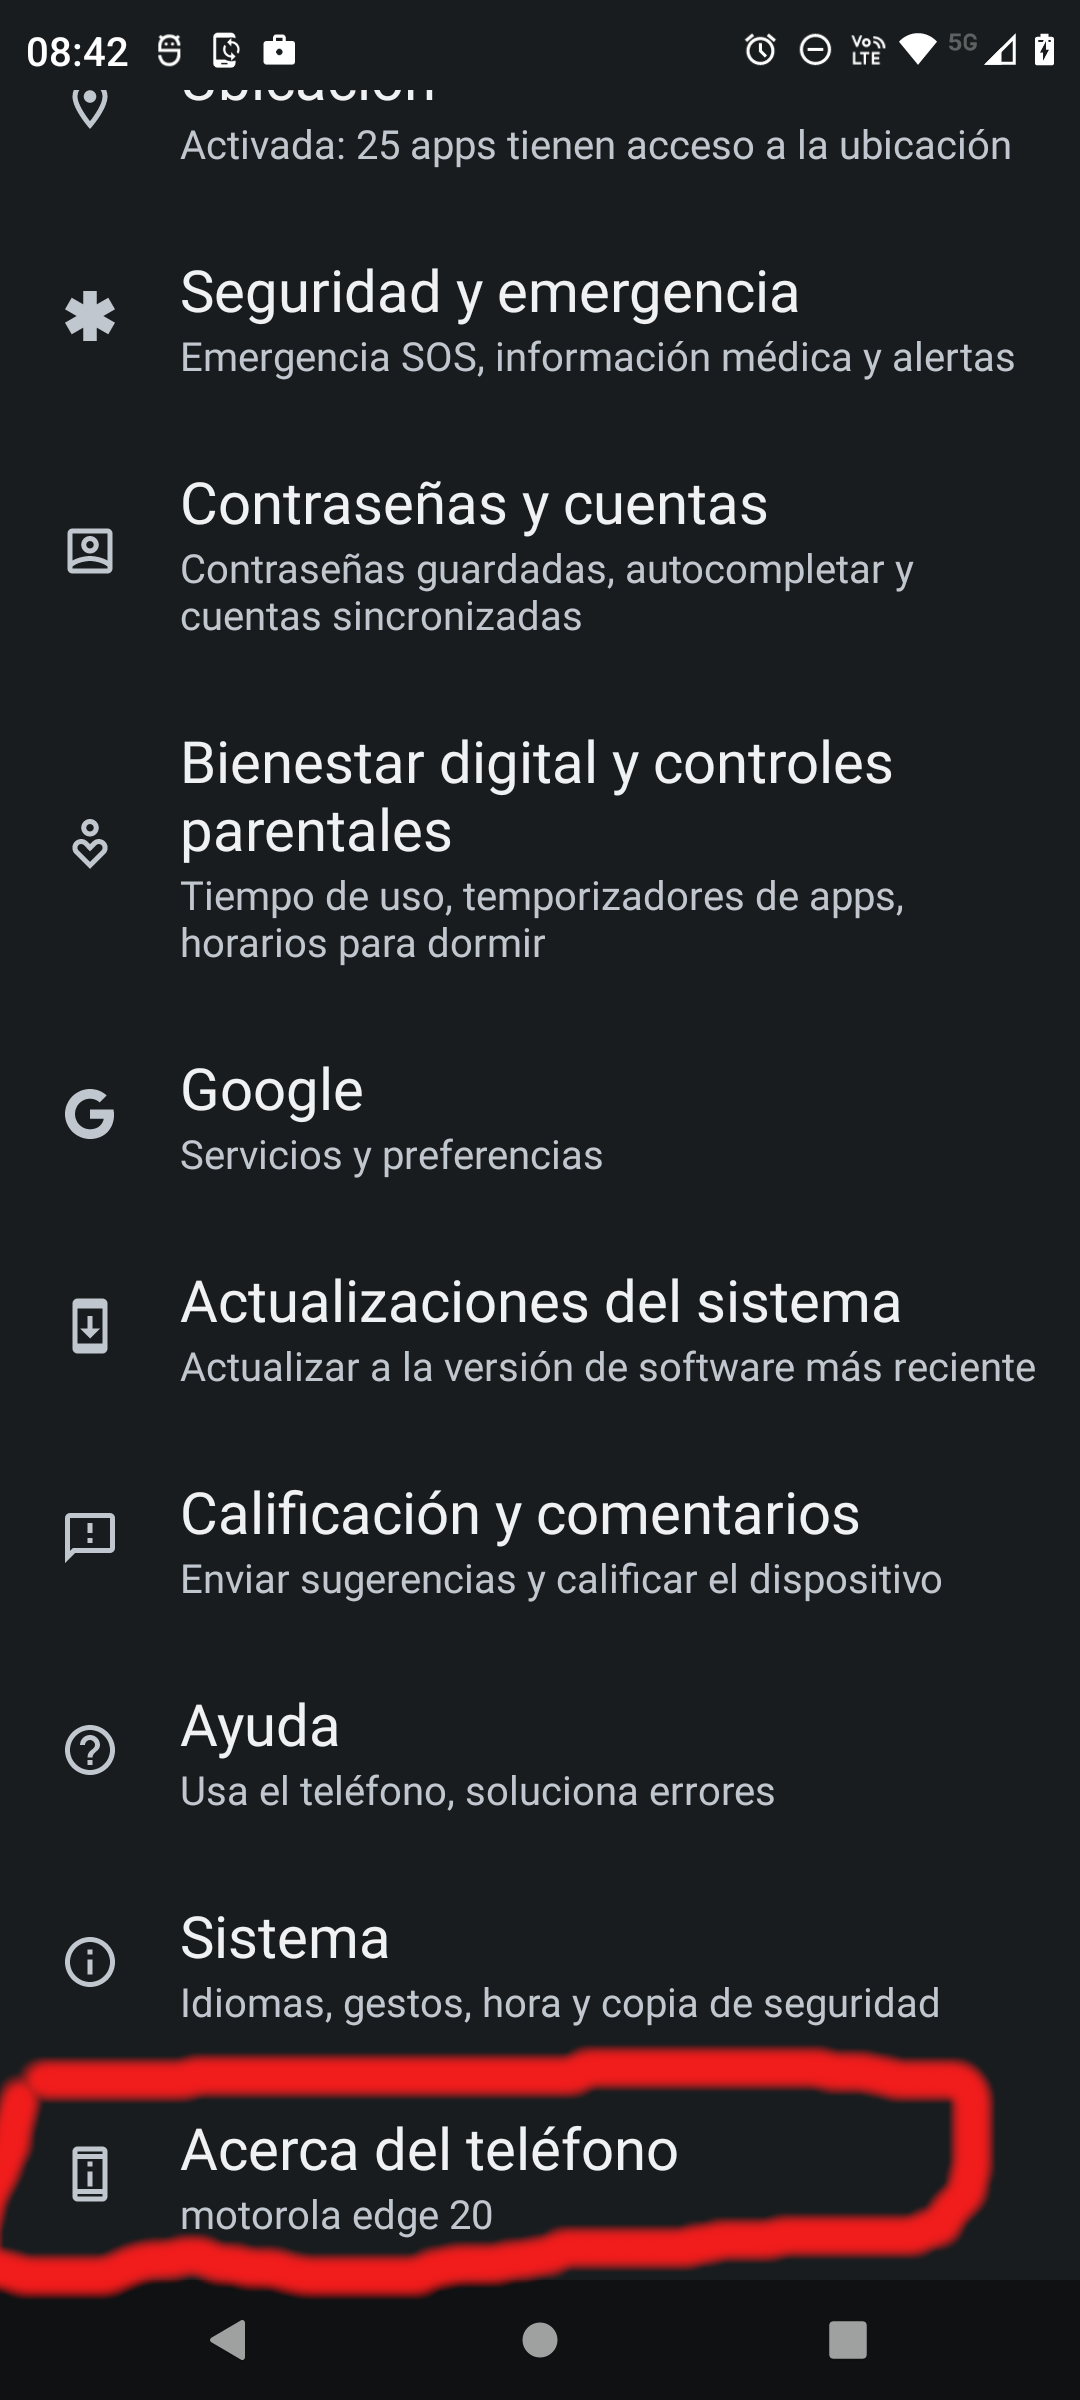
\includegraphics[width=0.95\linewidth]{01_Configurar/ModoDesarrollador3.png}    
\end{center}
\column{0.25\linewidth}
\begin{center}
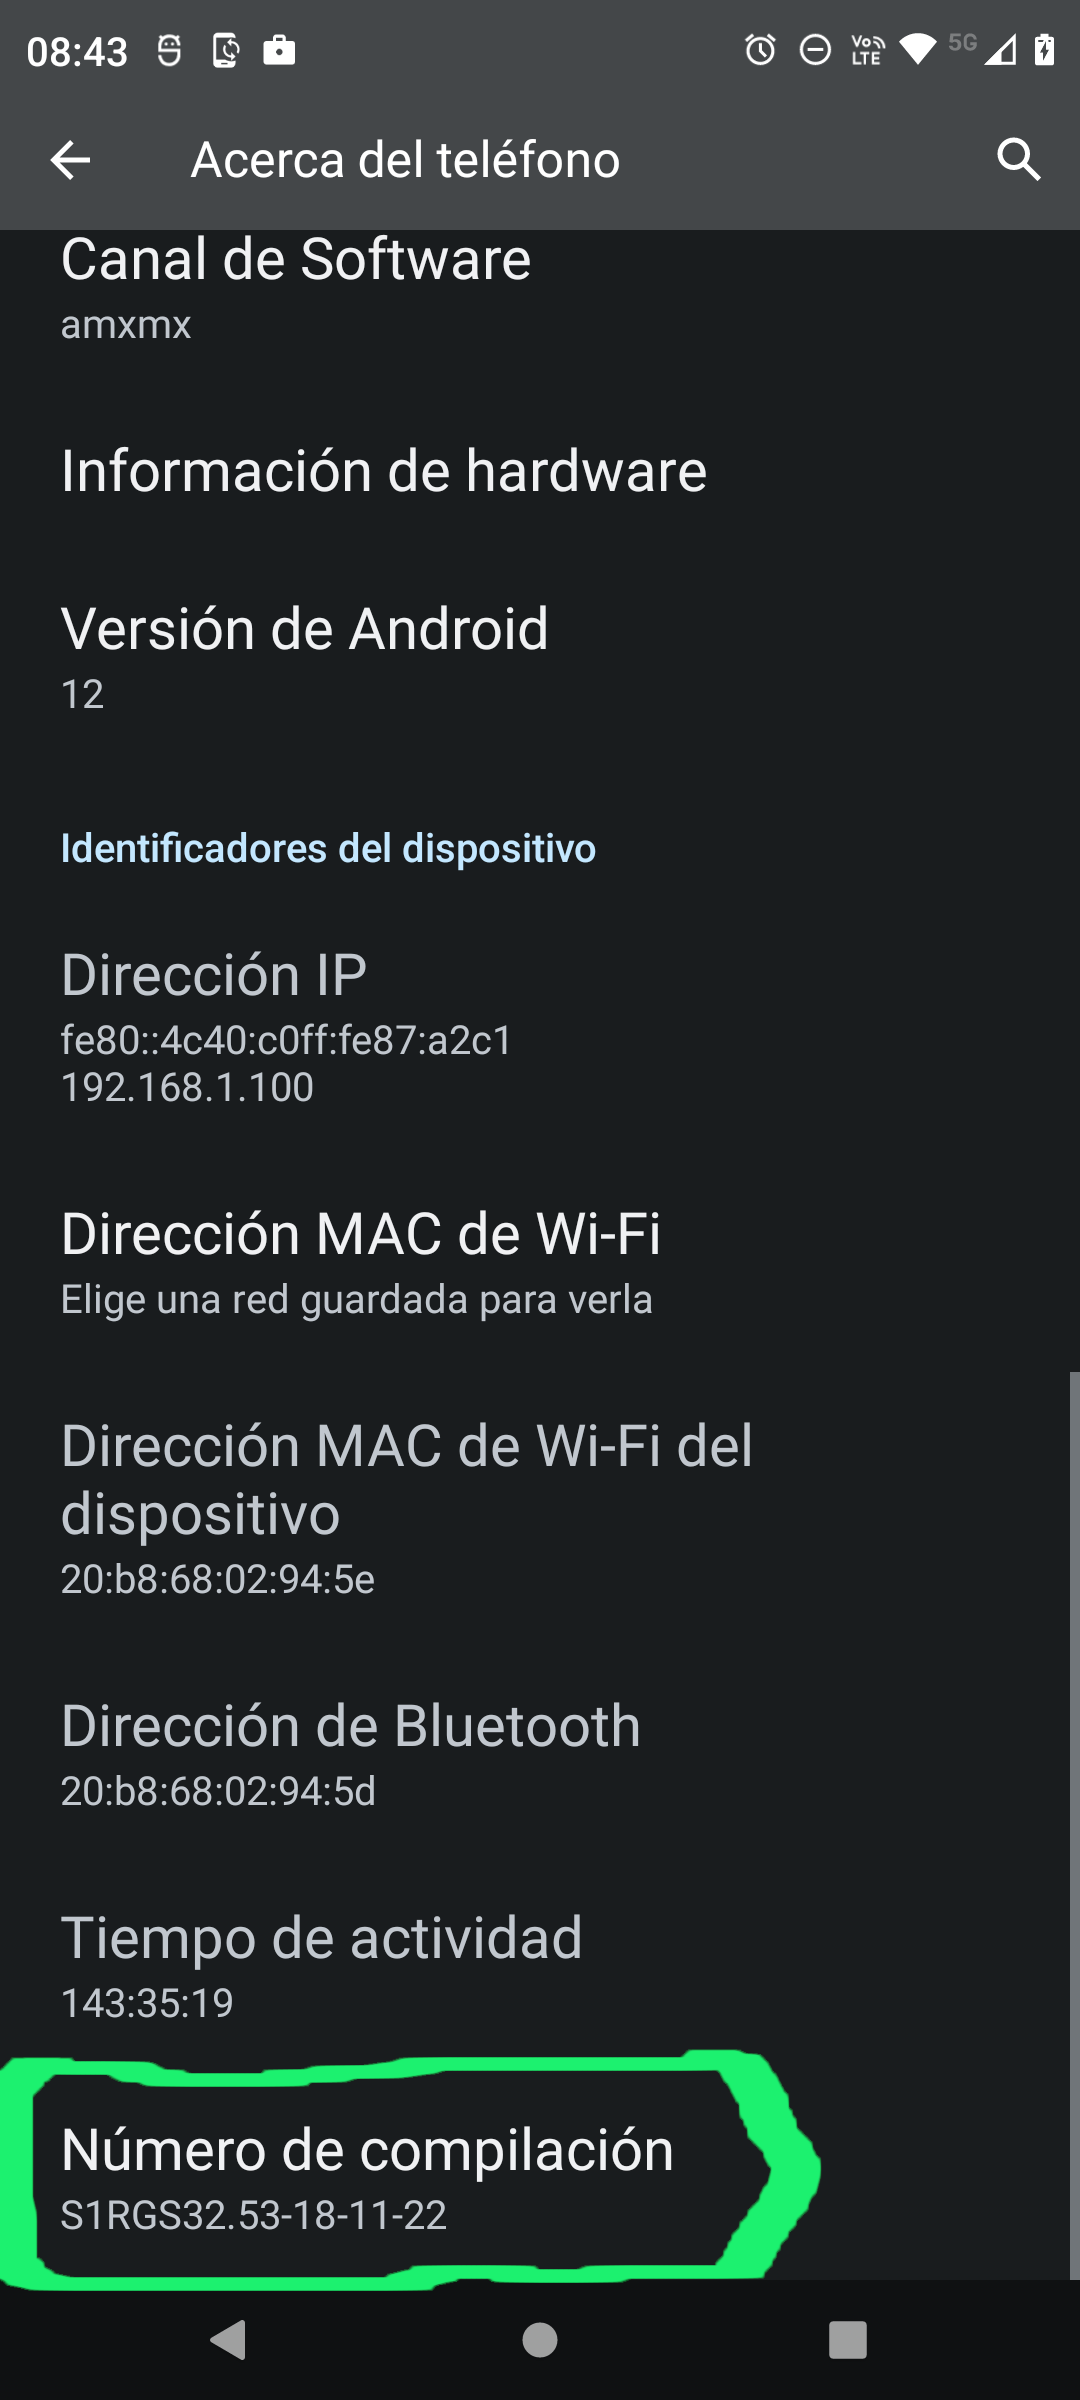
\includegraphics[width=0.95\linewidth]{01_Configurar/ModoDesarrollador4.png}    
\end{center}


\end{columns}

\end{frame}


\begin{frame}
\frametitle{Configurar telefono inteligente en modo de desarrollador (2)}  
\begin{columns}
\column{0.25\linewidth}
\begin{center}
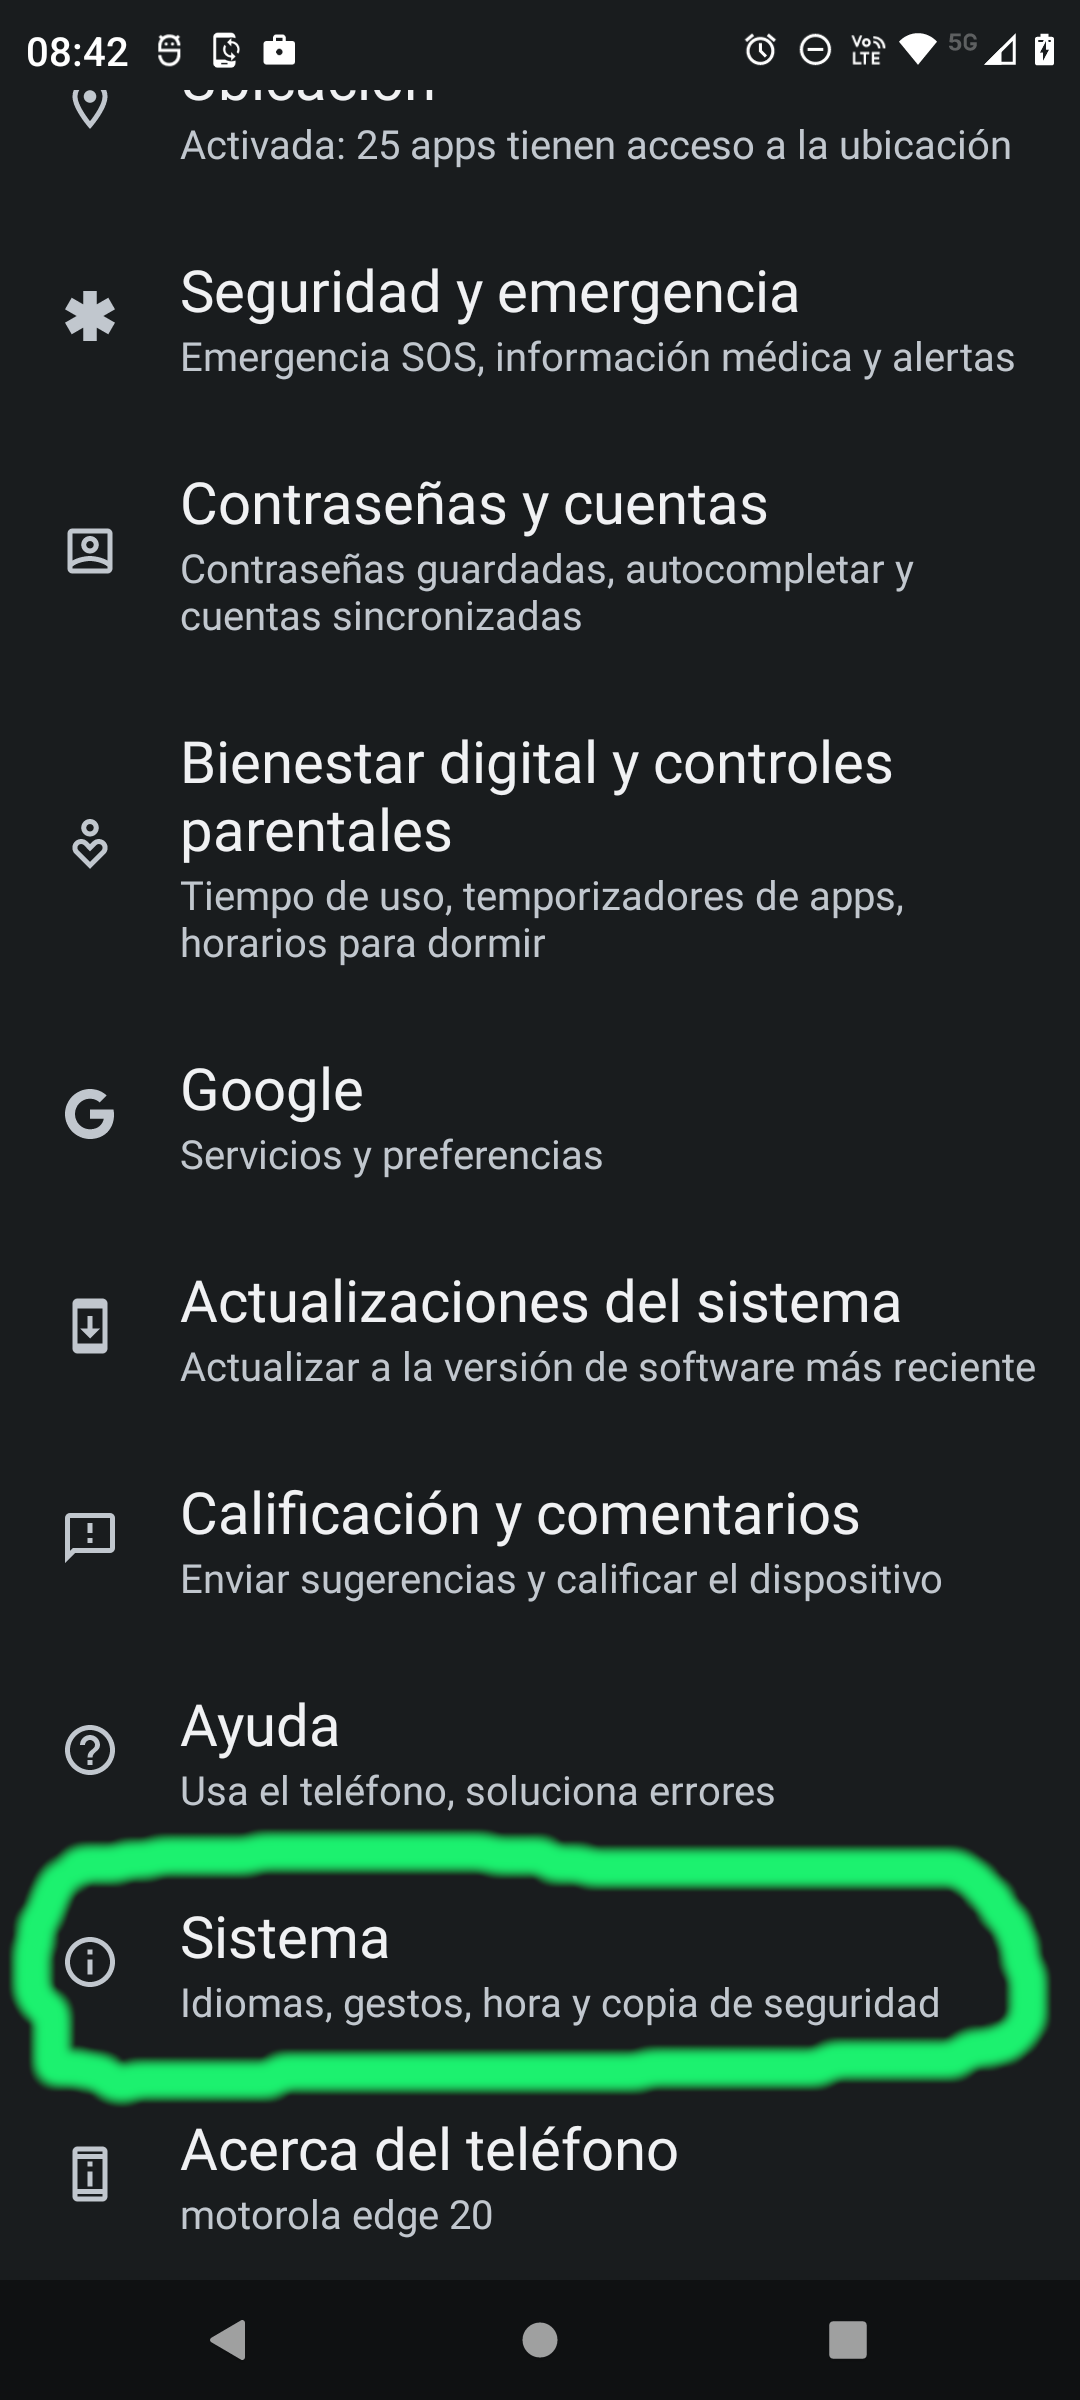
\includegraphics[width=0.95\linewidth]{01_Configurar/ModoDesarrollador5.png}    
\end{center}
\column{0.25\linewidth}
\begin{center}
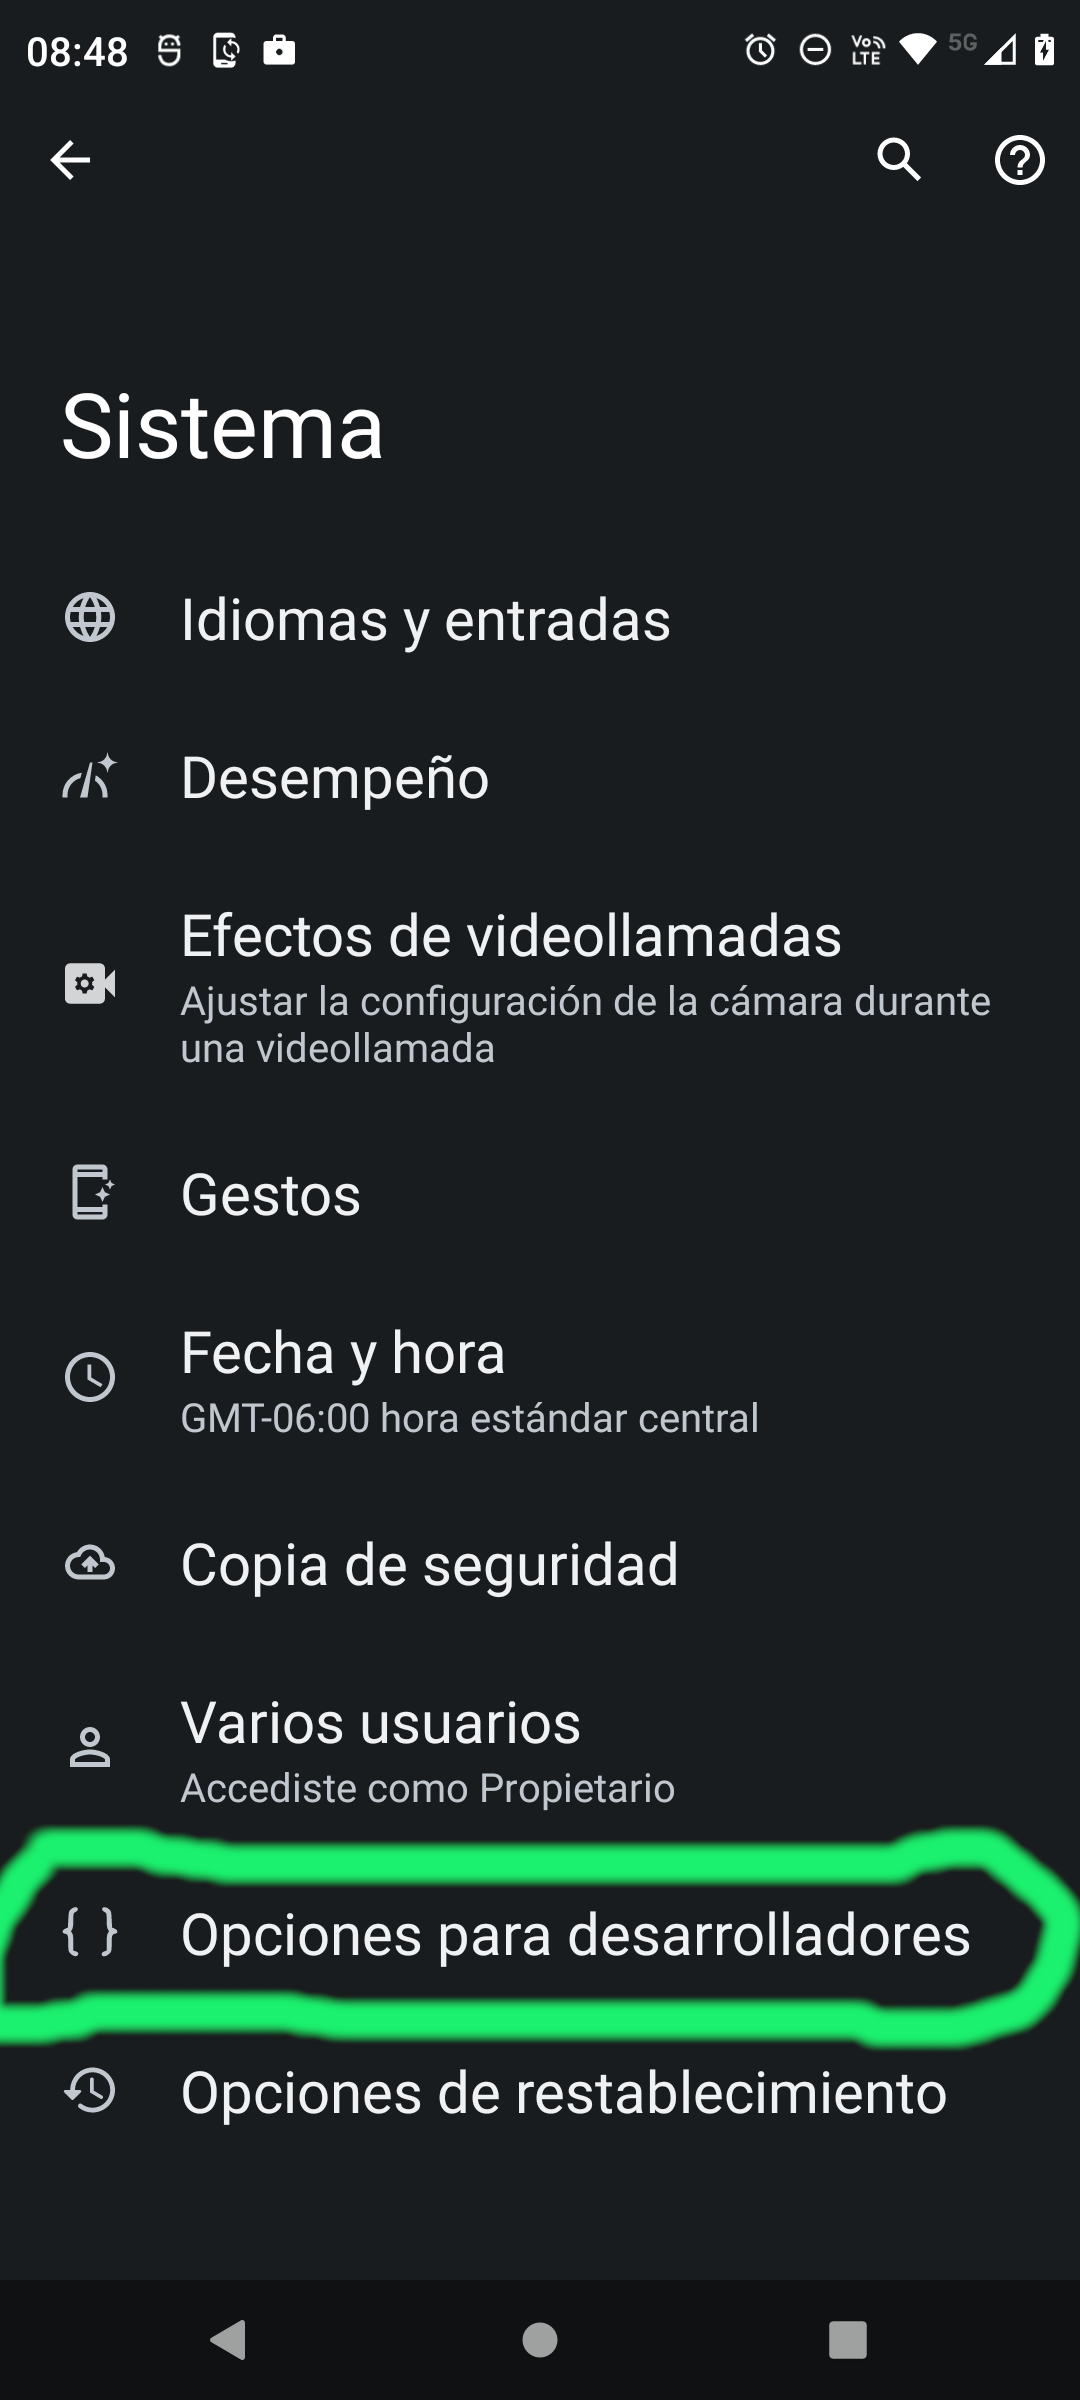
\includegraphics[width=0.95\linewidth]{01_Configurar/ModoDesarrollador6.png}    
\end{center}
\column{0.25\linewidth}
\begin{center}
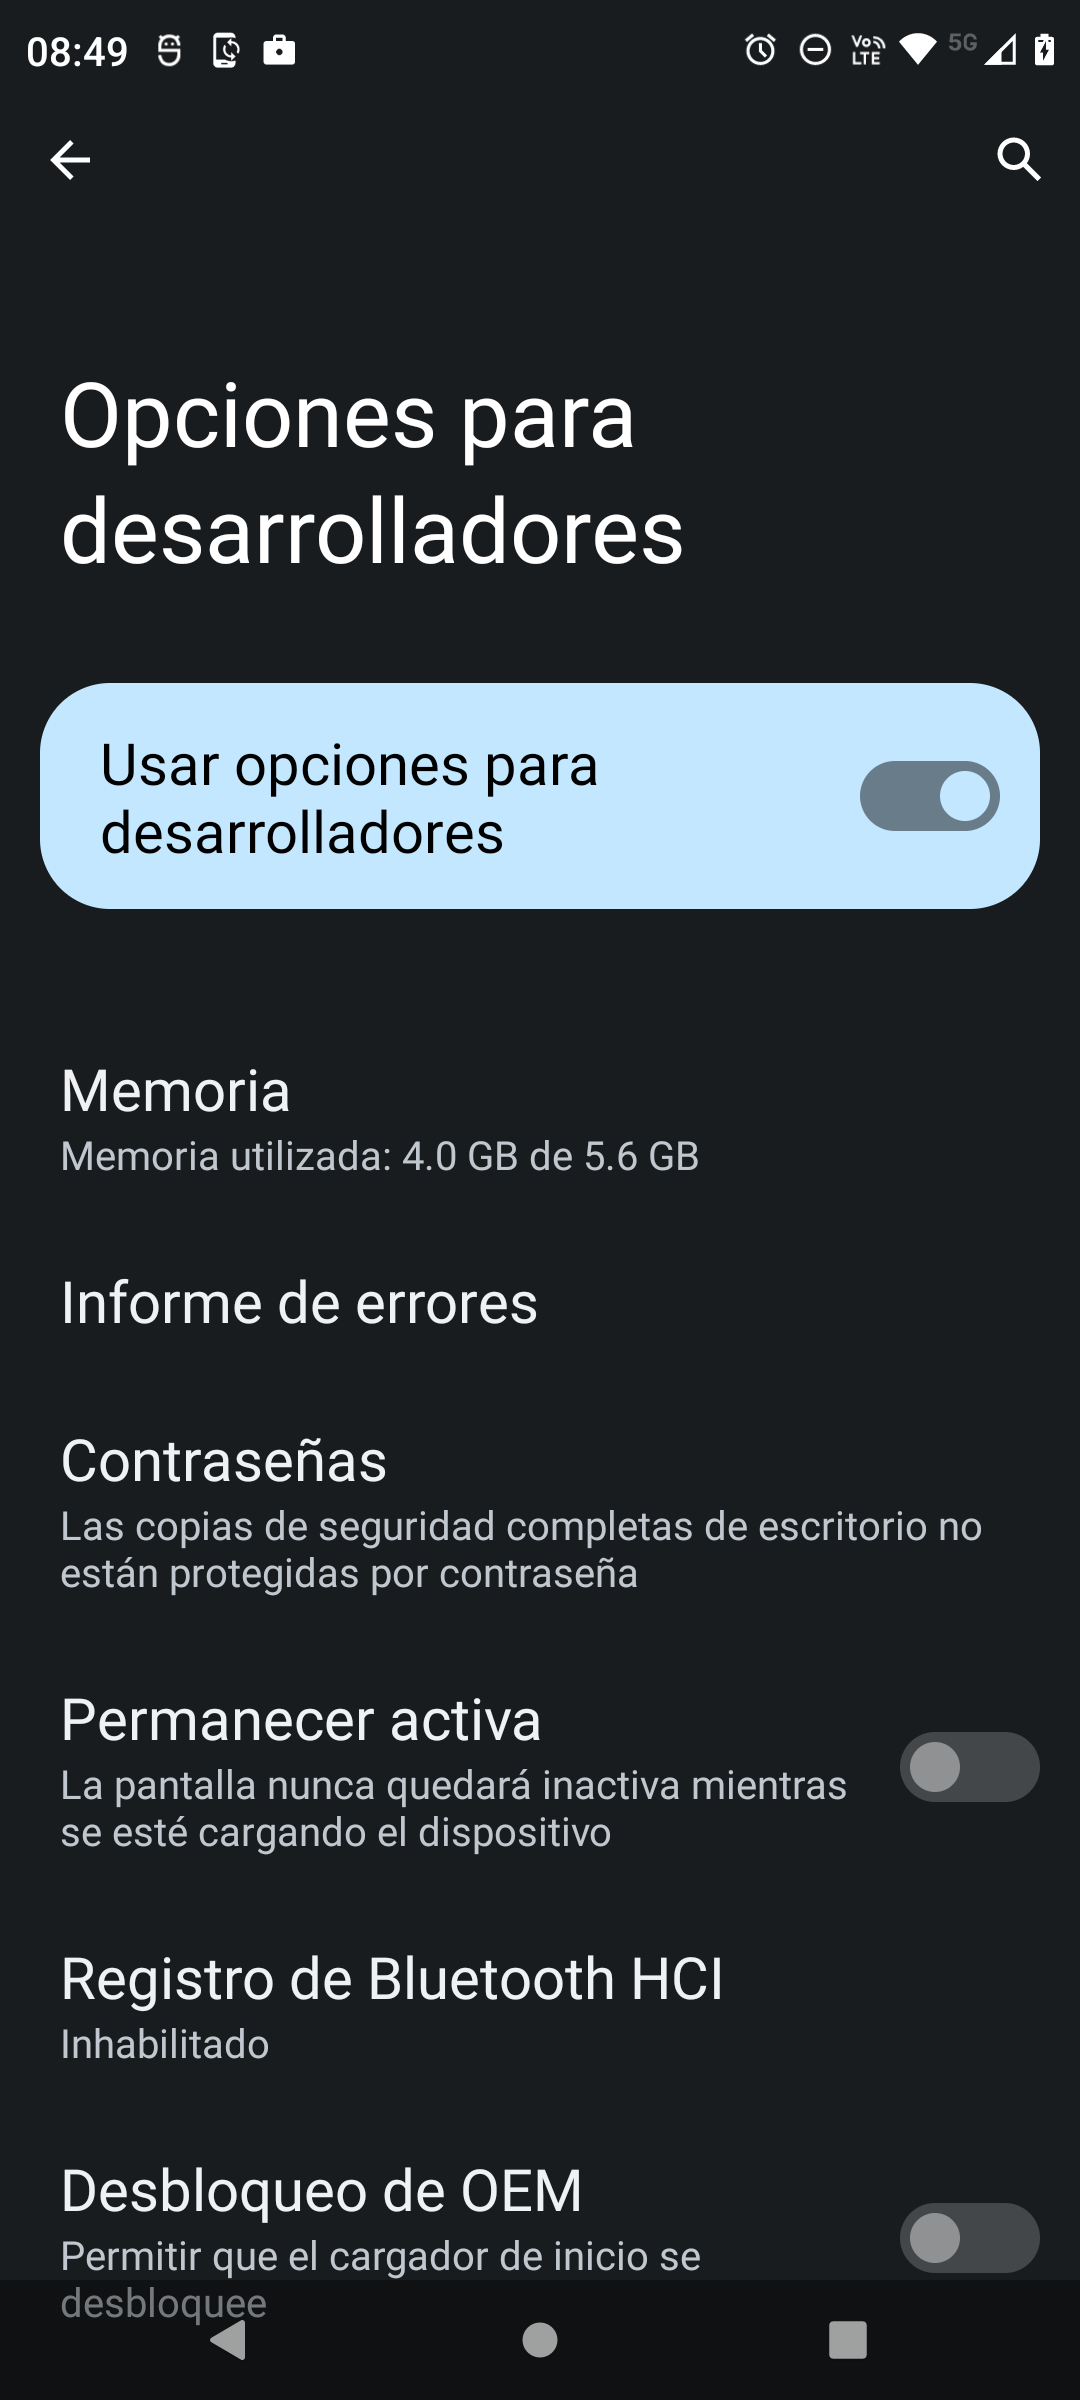
\includegraphics[width=0.95\linewidth]{01_Configurar/ModoDesarrollador7.png}    
\end{center}
\column{0.25\linewidth}
\begin{center}
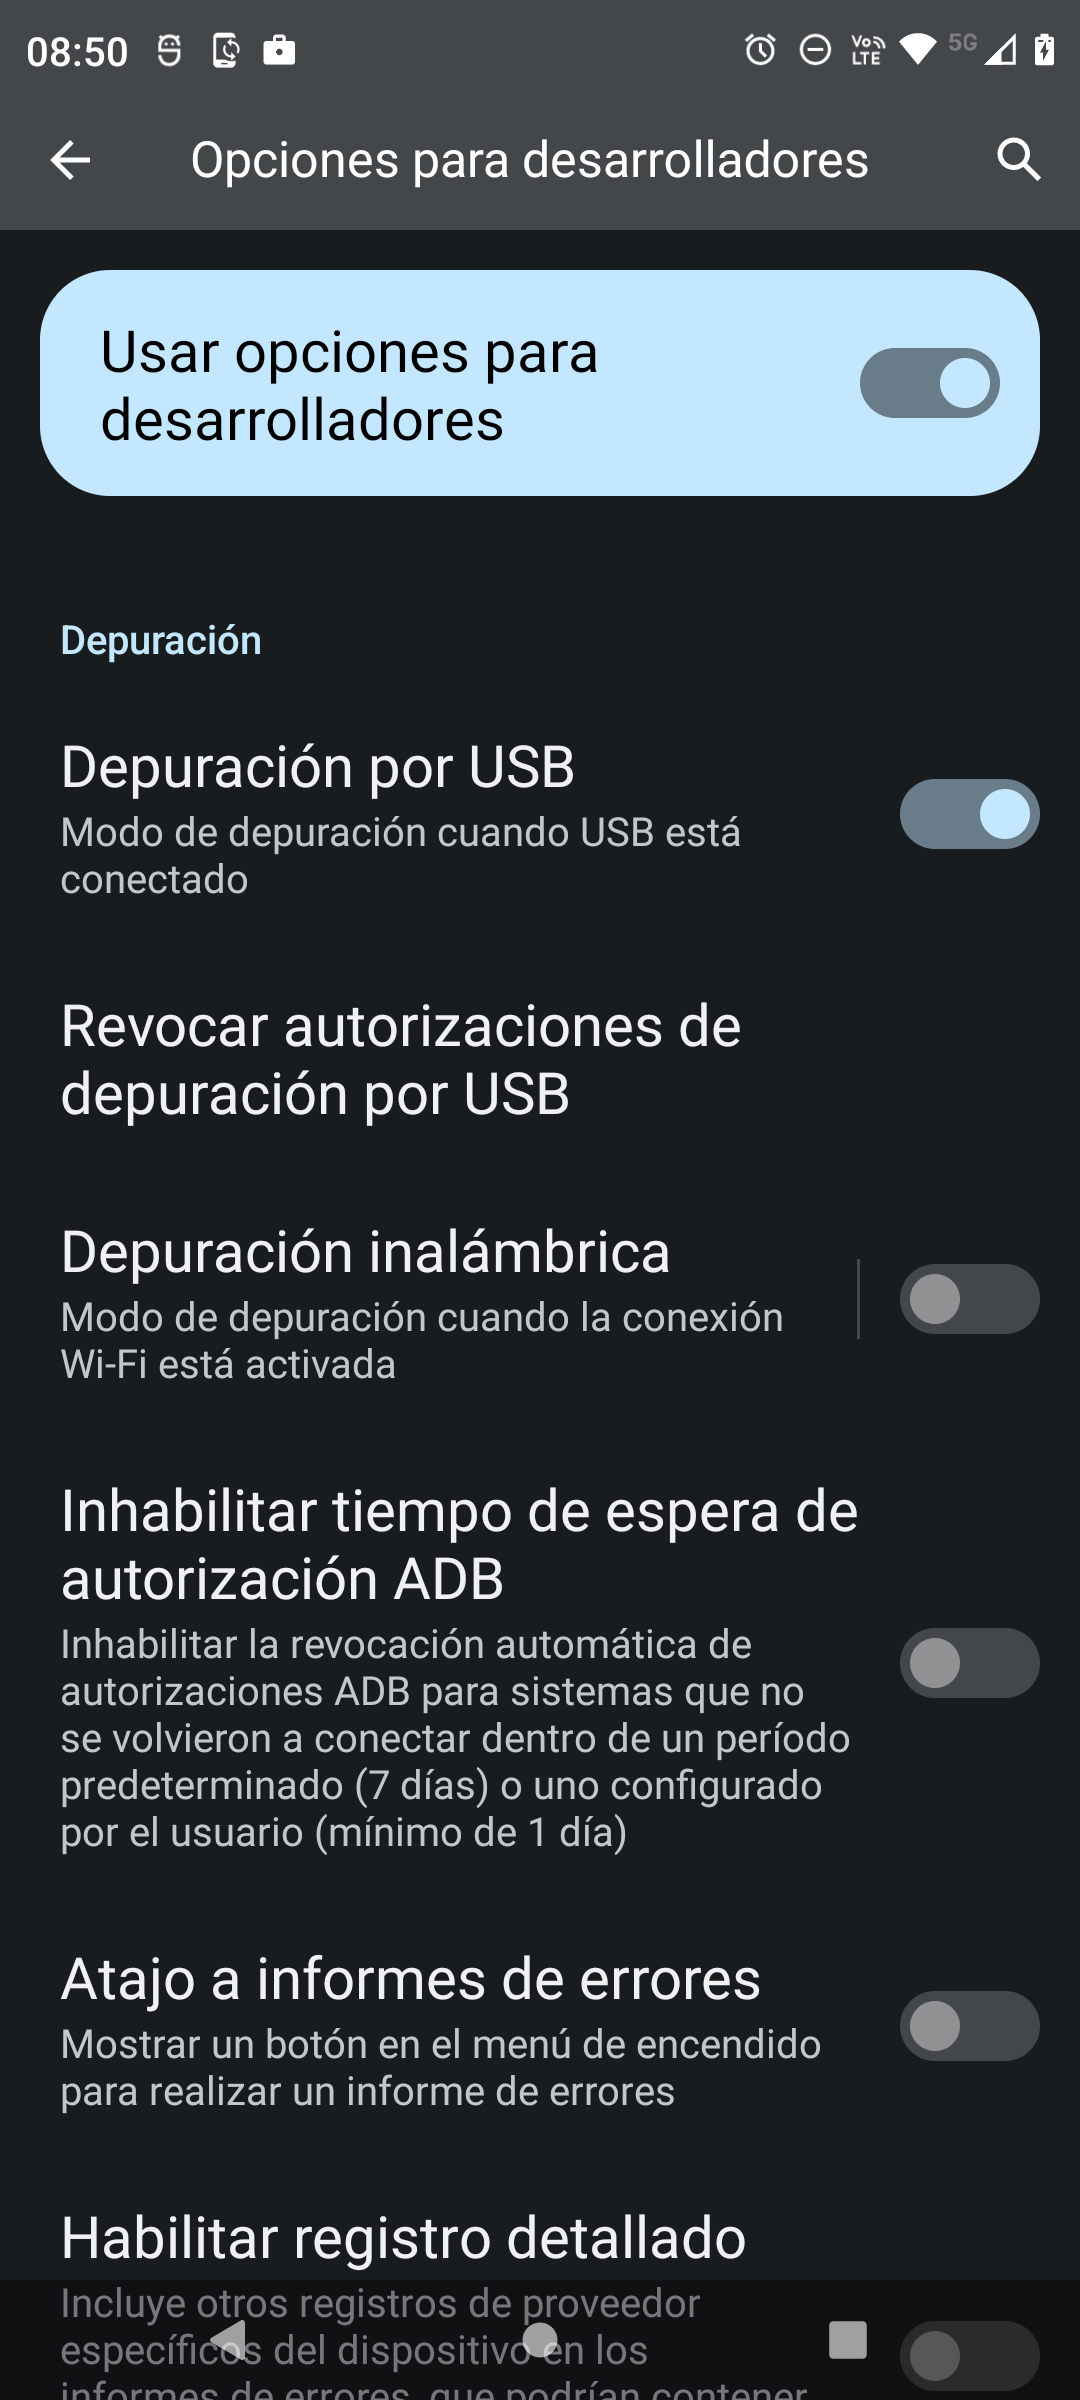
\includegraphics[width=0.95\linewidth]{01_Configurar/ModoDesarrollador8.png}    
\end{center}
\end{columns}
\end{frame}

\begin{frame}
\frametitle{Configurar telefono inteligente en modo de desarrollador (3)}  
\begin{columns}
\column{0.75\linewidth}

\begin{itemize}
\item Al habilitar la depuracion, aparece un mensaje de advertencia
\item Una vez que hayas terminado tus pruebas, se recomienda deshabilitar este modo de depuraci\'on
\item Para poder instalar una aplicaci\'on desarrollada con Android Studio, se debe conectar el tel\'efono inteligente a la computadora usando un cable USB
\end{itemize}

\column{0.25\linewidth}
\begin{center}
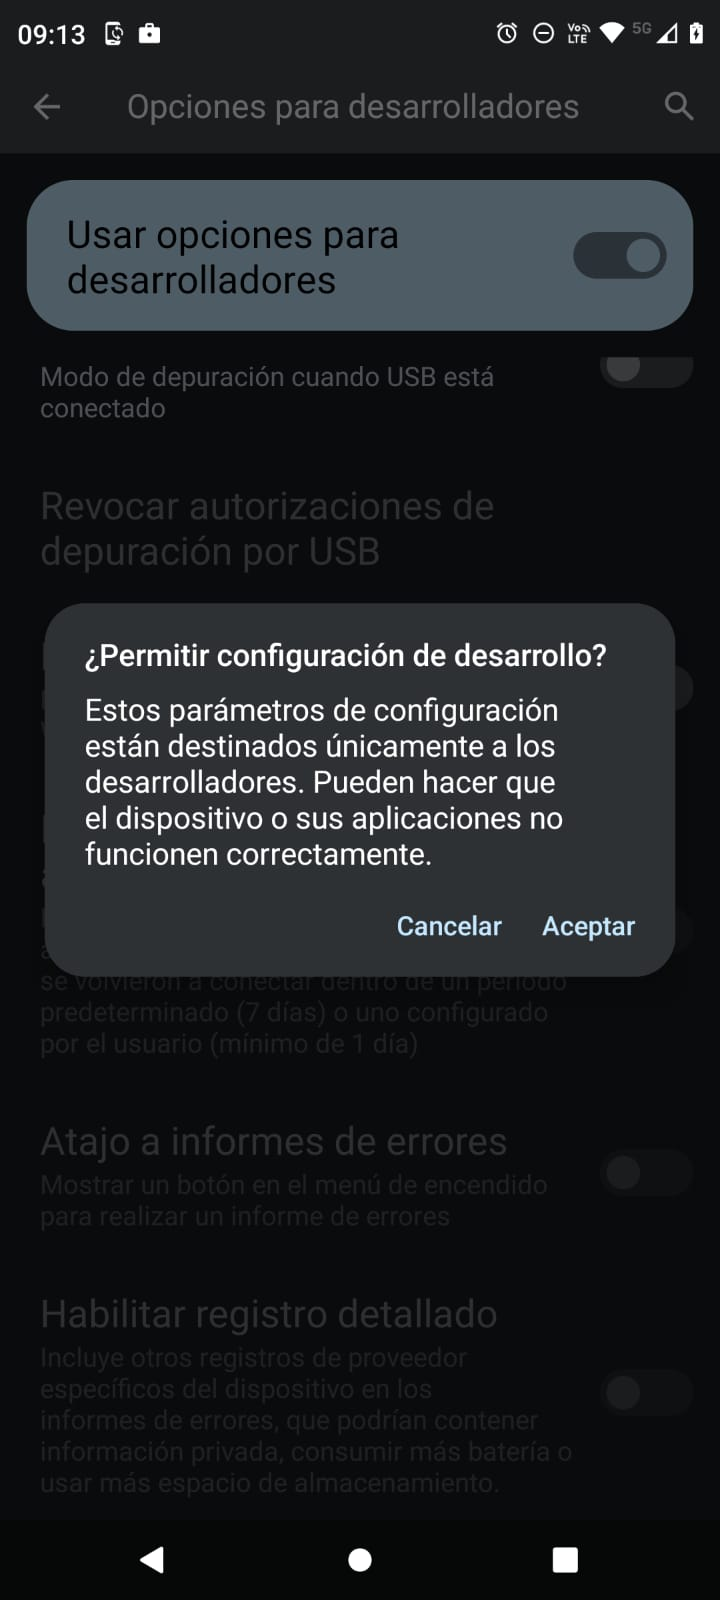
\includegraphics[width=0.95\linewidth]{01_Configurar/PermitirHabiliarOpcionesDesarrollo.jpg}    
\end{center}
\end{columns}
\end{frame}



\begin{frame}
\frametitle{Conectar smartphone a la computadora (Cable USB)}  
\begin{columns}
\column{0.25\linewidth}
\begin{itemize}
\item Al conectar el dispositivo por primera vez, aparece un mensaje de confirmaci\'on en el dispositivo
\item Configurar el telefono para que se conecte en modo de transferencia de archivos (por defecto, esta cargando)
\end{itemize}

\column{0.25\linewidth}
\begin{center}
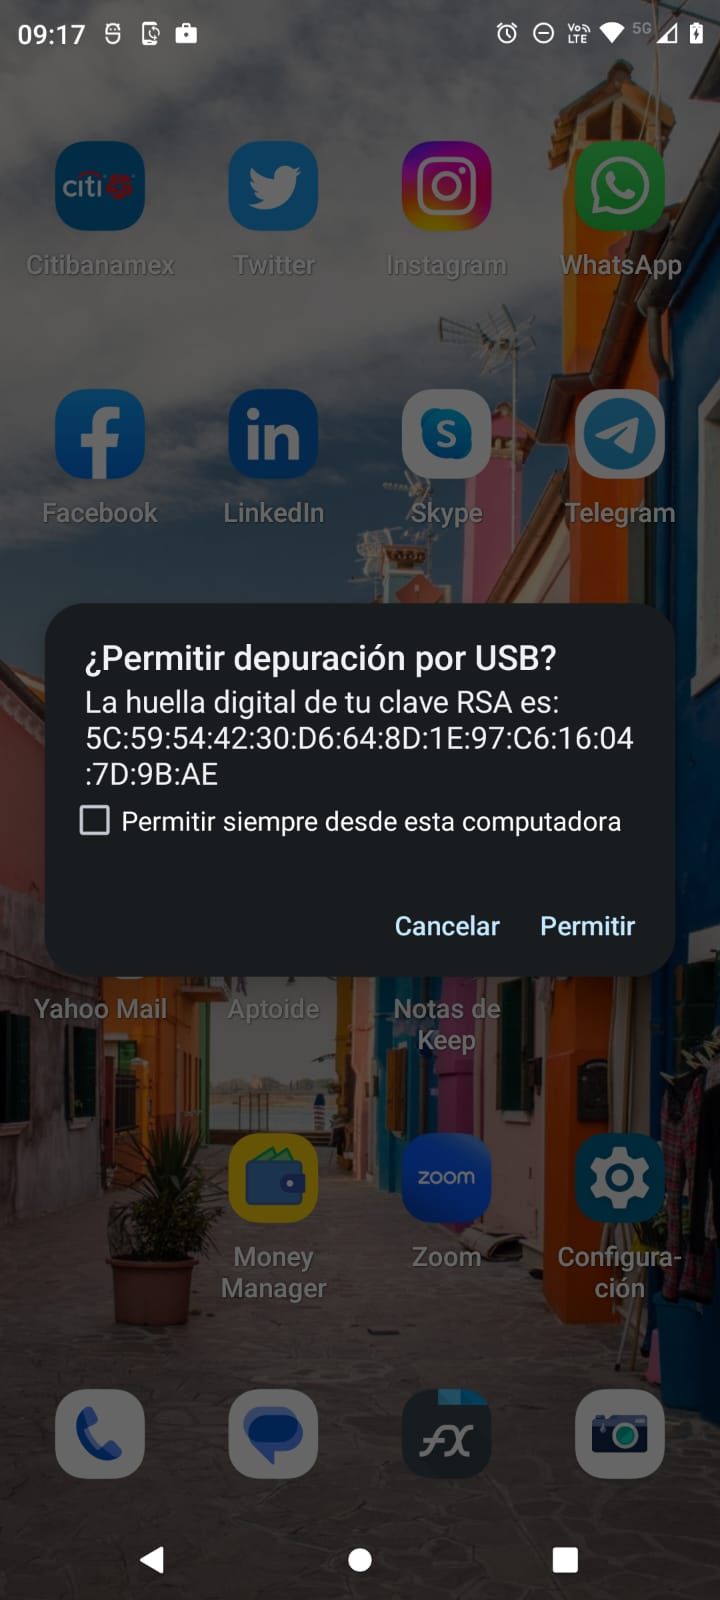
\includegraphics[width=0.95\linewidth]{01_Configurar/HabilitarDepuracionUSB2.jpg}    
\end{center}

\column{0.25\linewidth}
\begin{center}
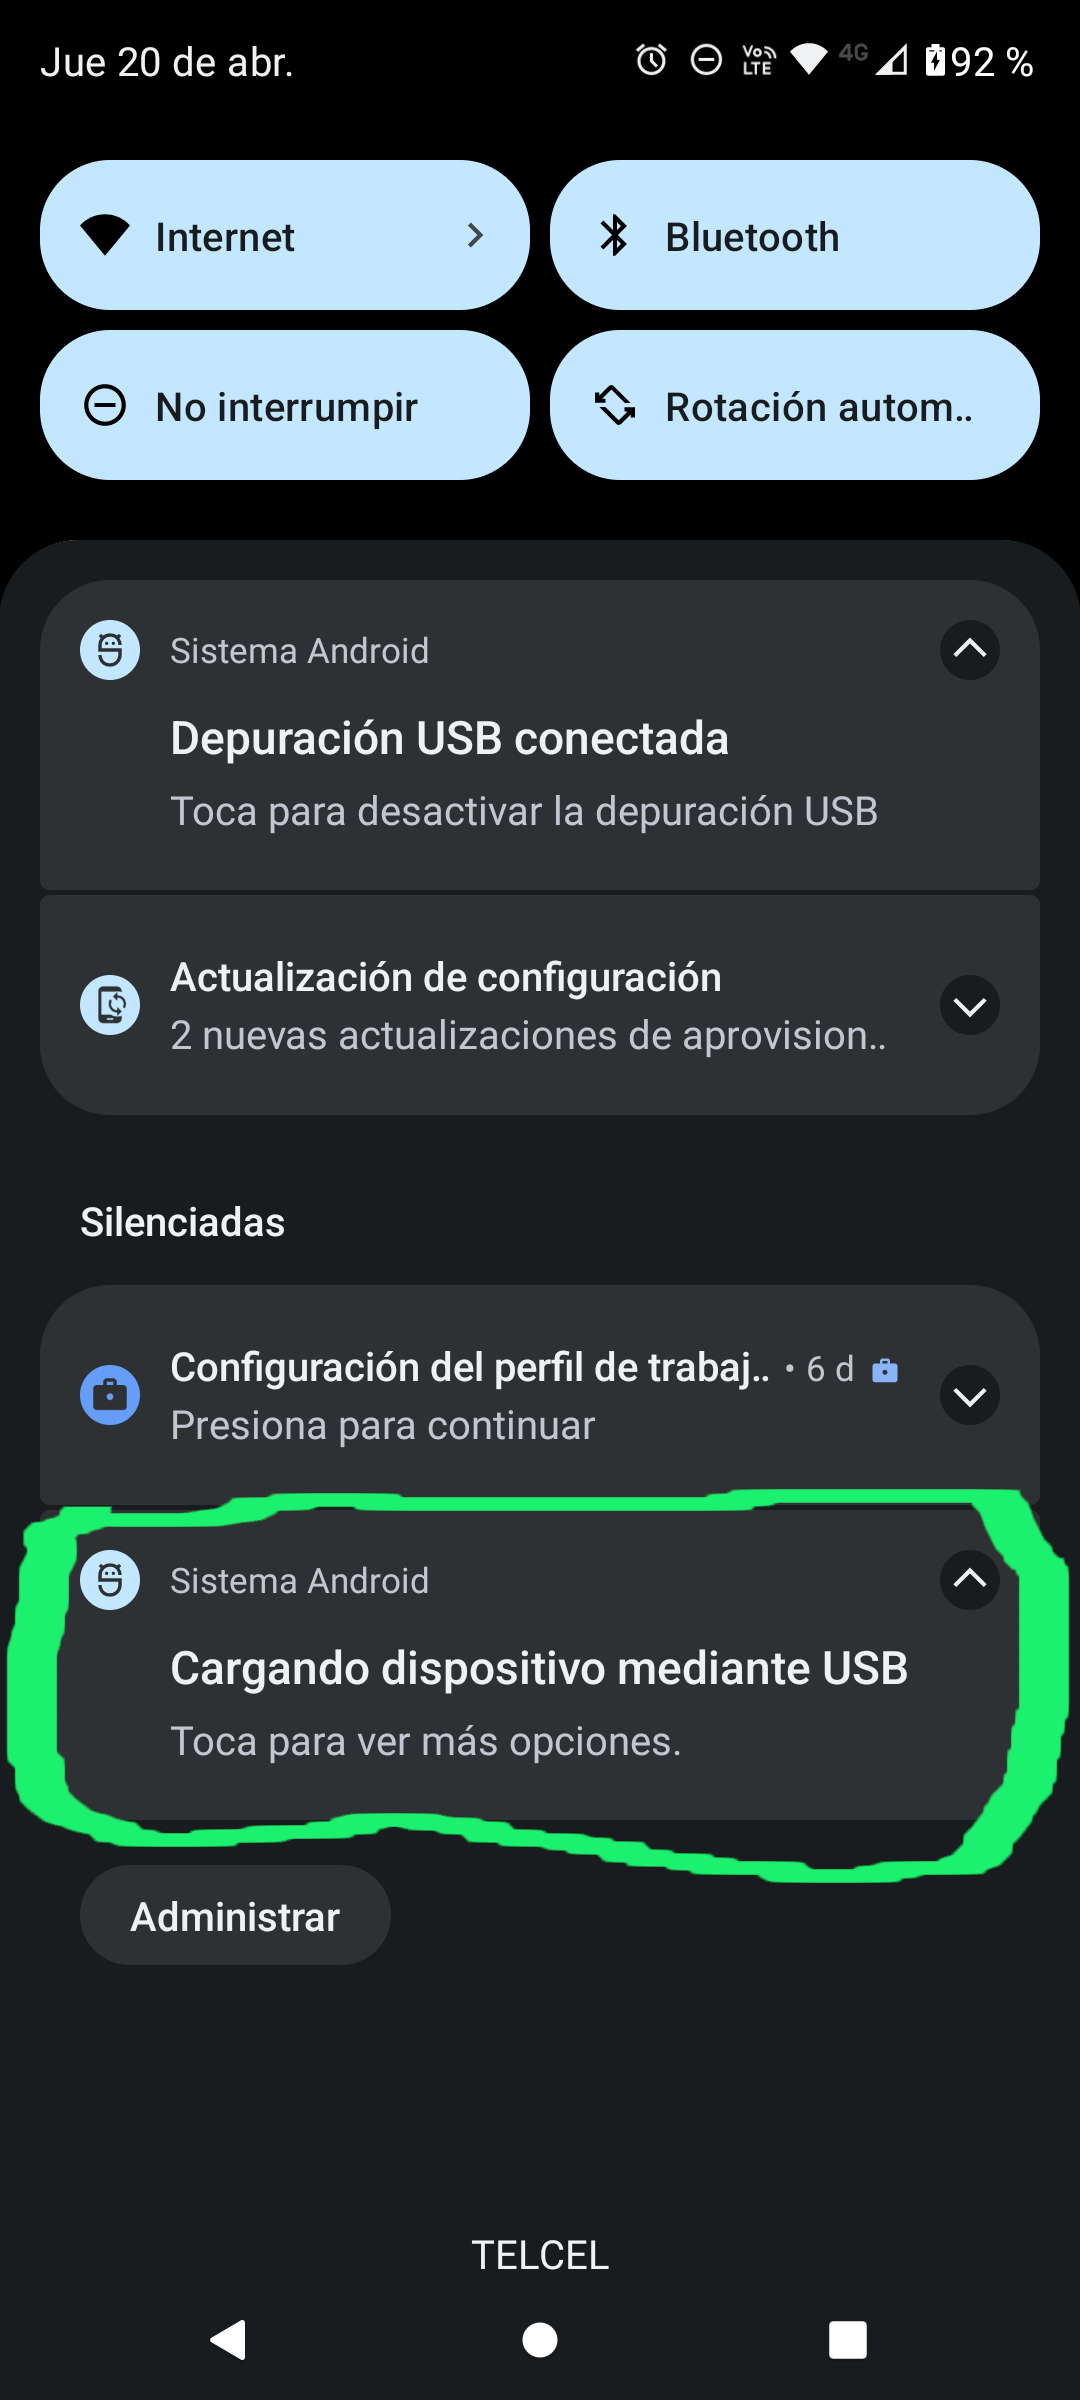
\includegraphics[width=0.95\linewidth]{01_Configurar/ModoConexion1.png}    
\end{center}

\column{0.25\linewidth}
\begin{center}
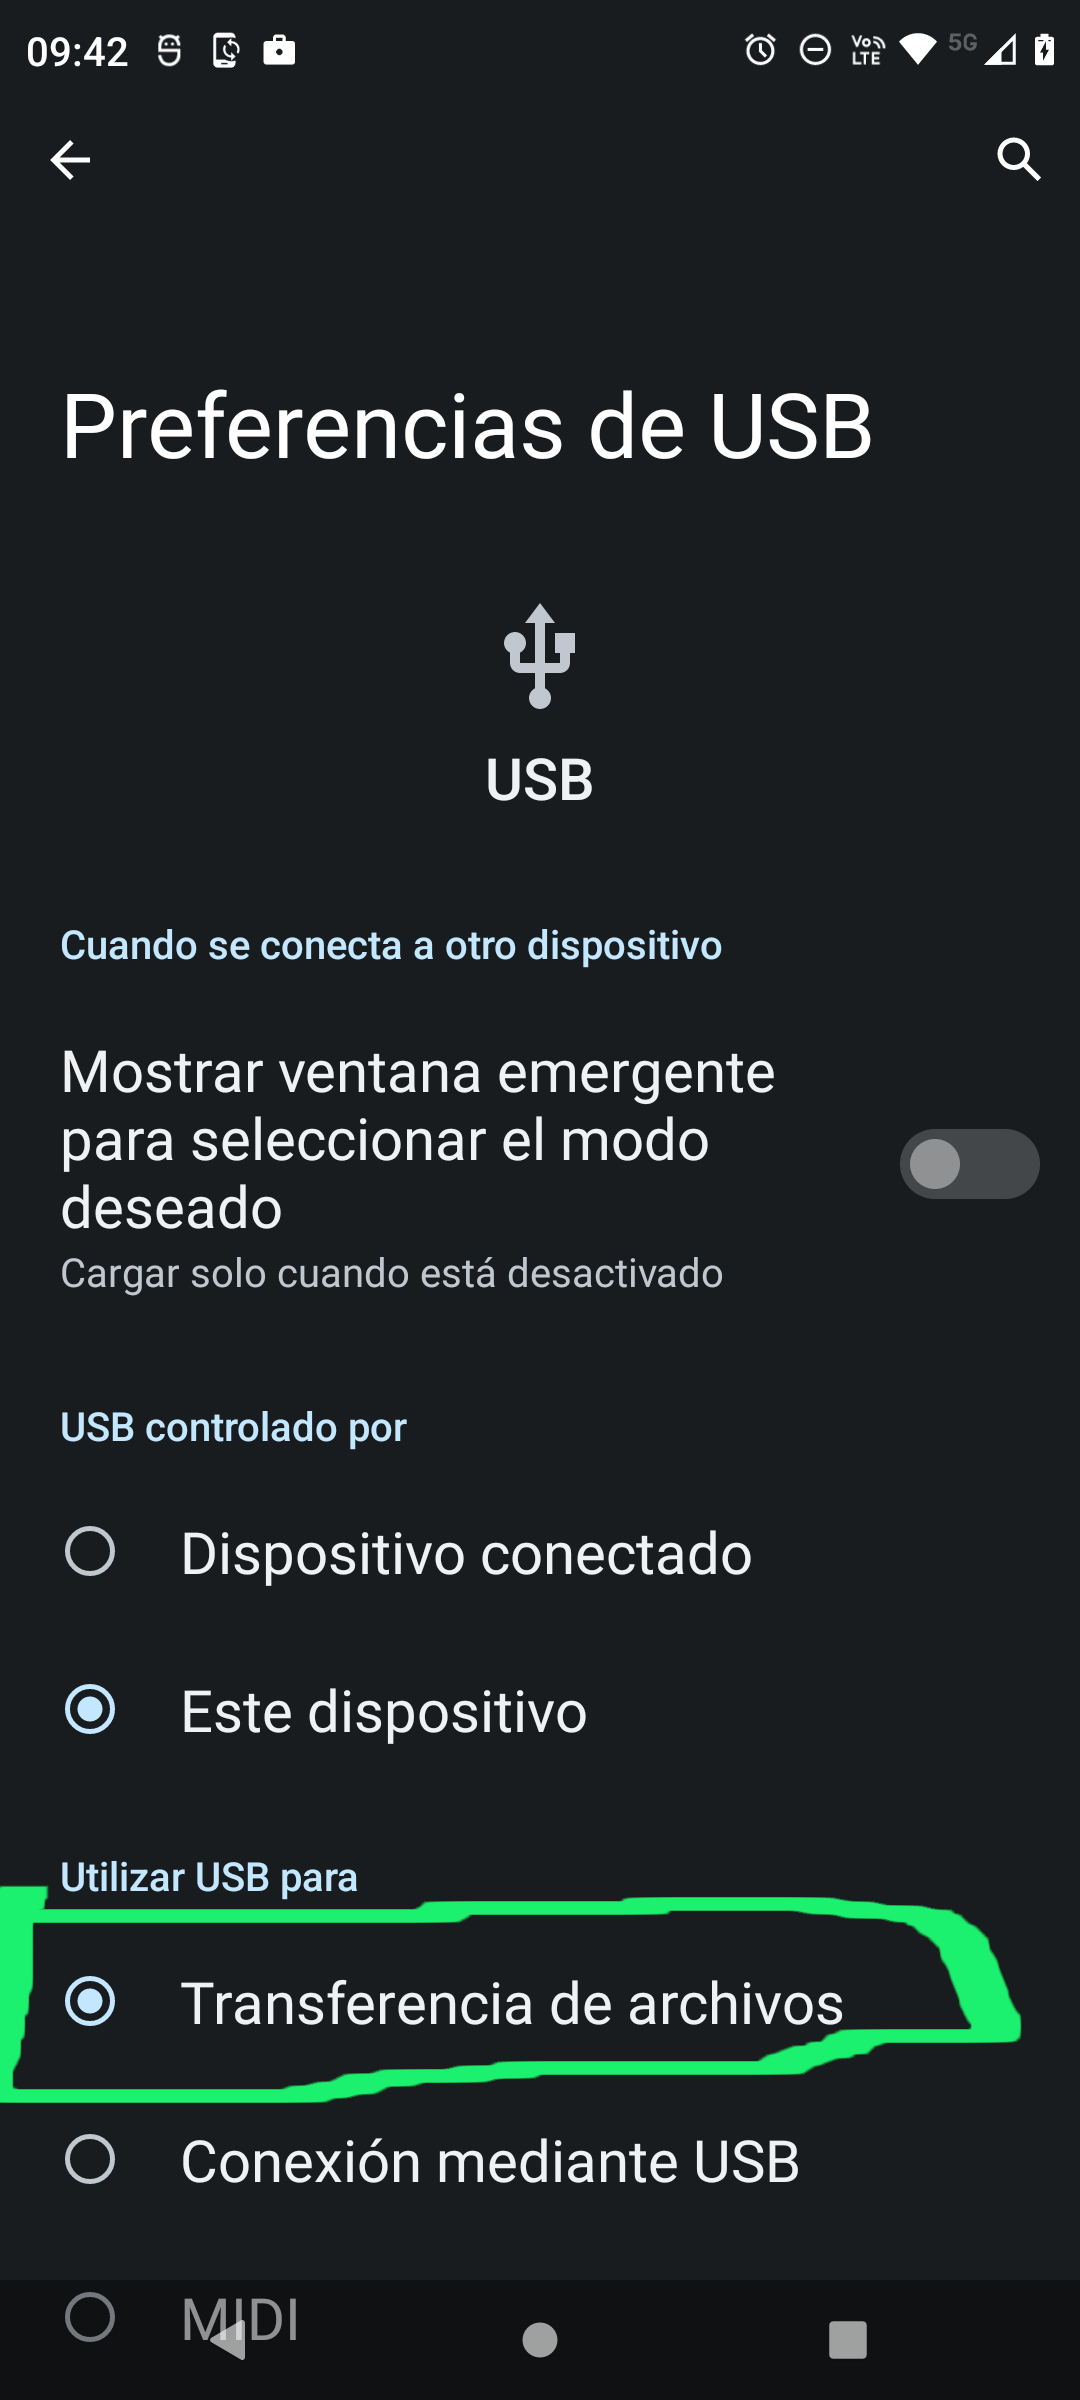
\includegraphics[width=0.95\linewidth]{01_Configurar/ModoConexion2.png}    
\end{center}
\end{columns}
\end{frame}



\begin{frame}
\frametitle{Ejecutar proyecto en telefono inteligente} 
\begin{columns}

\column{0.75\linewidth}
\begin{itemize}
\item Una vez conectado el telefono, debe aparecer el modelo en la parte superior (lado derecho) de tu proyecto de Android Studio
\item Para instalar la aplicacion en el telefono, deber dar click en una flecha verde justo a un lado de nombre del telefono (sean pacientes, puede tardar un poco la primera vez)
\end{itemize}
\begin{center}
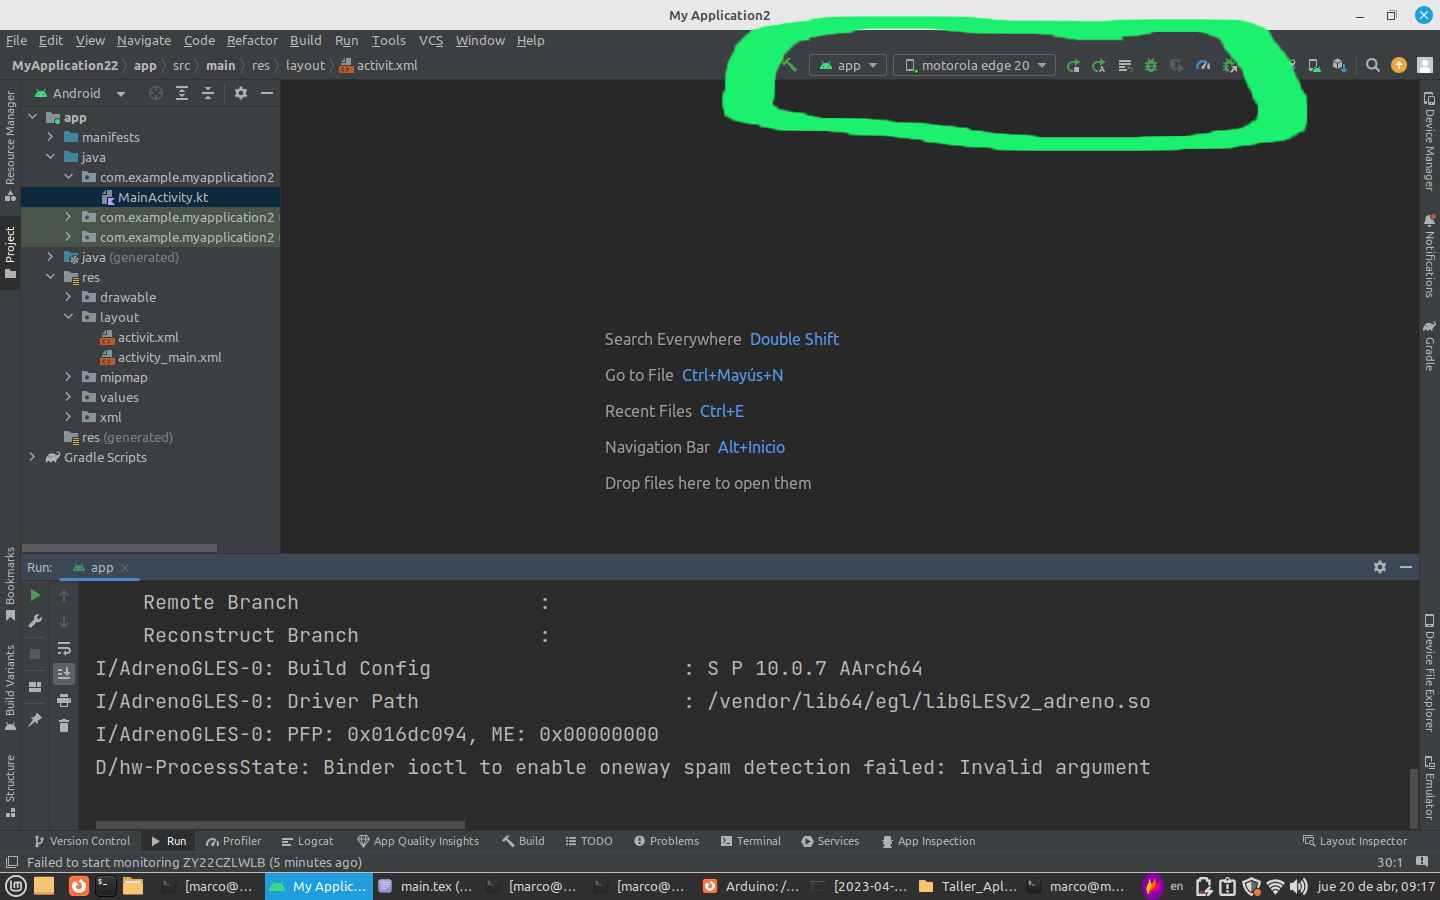
\includegraphics[width=0.65\linewidth]{01_Configurar/AndroidStudio_SmartphoneReconocido.png}    
\end{center}
\column{0.25\linewidth}
\begin{center}
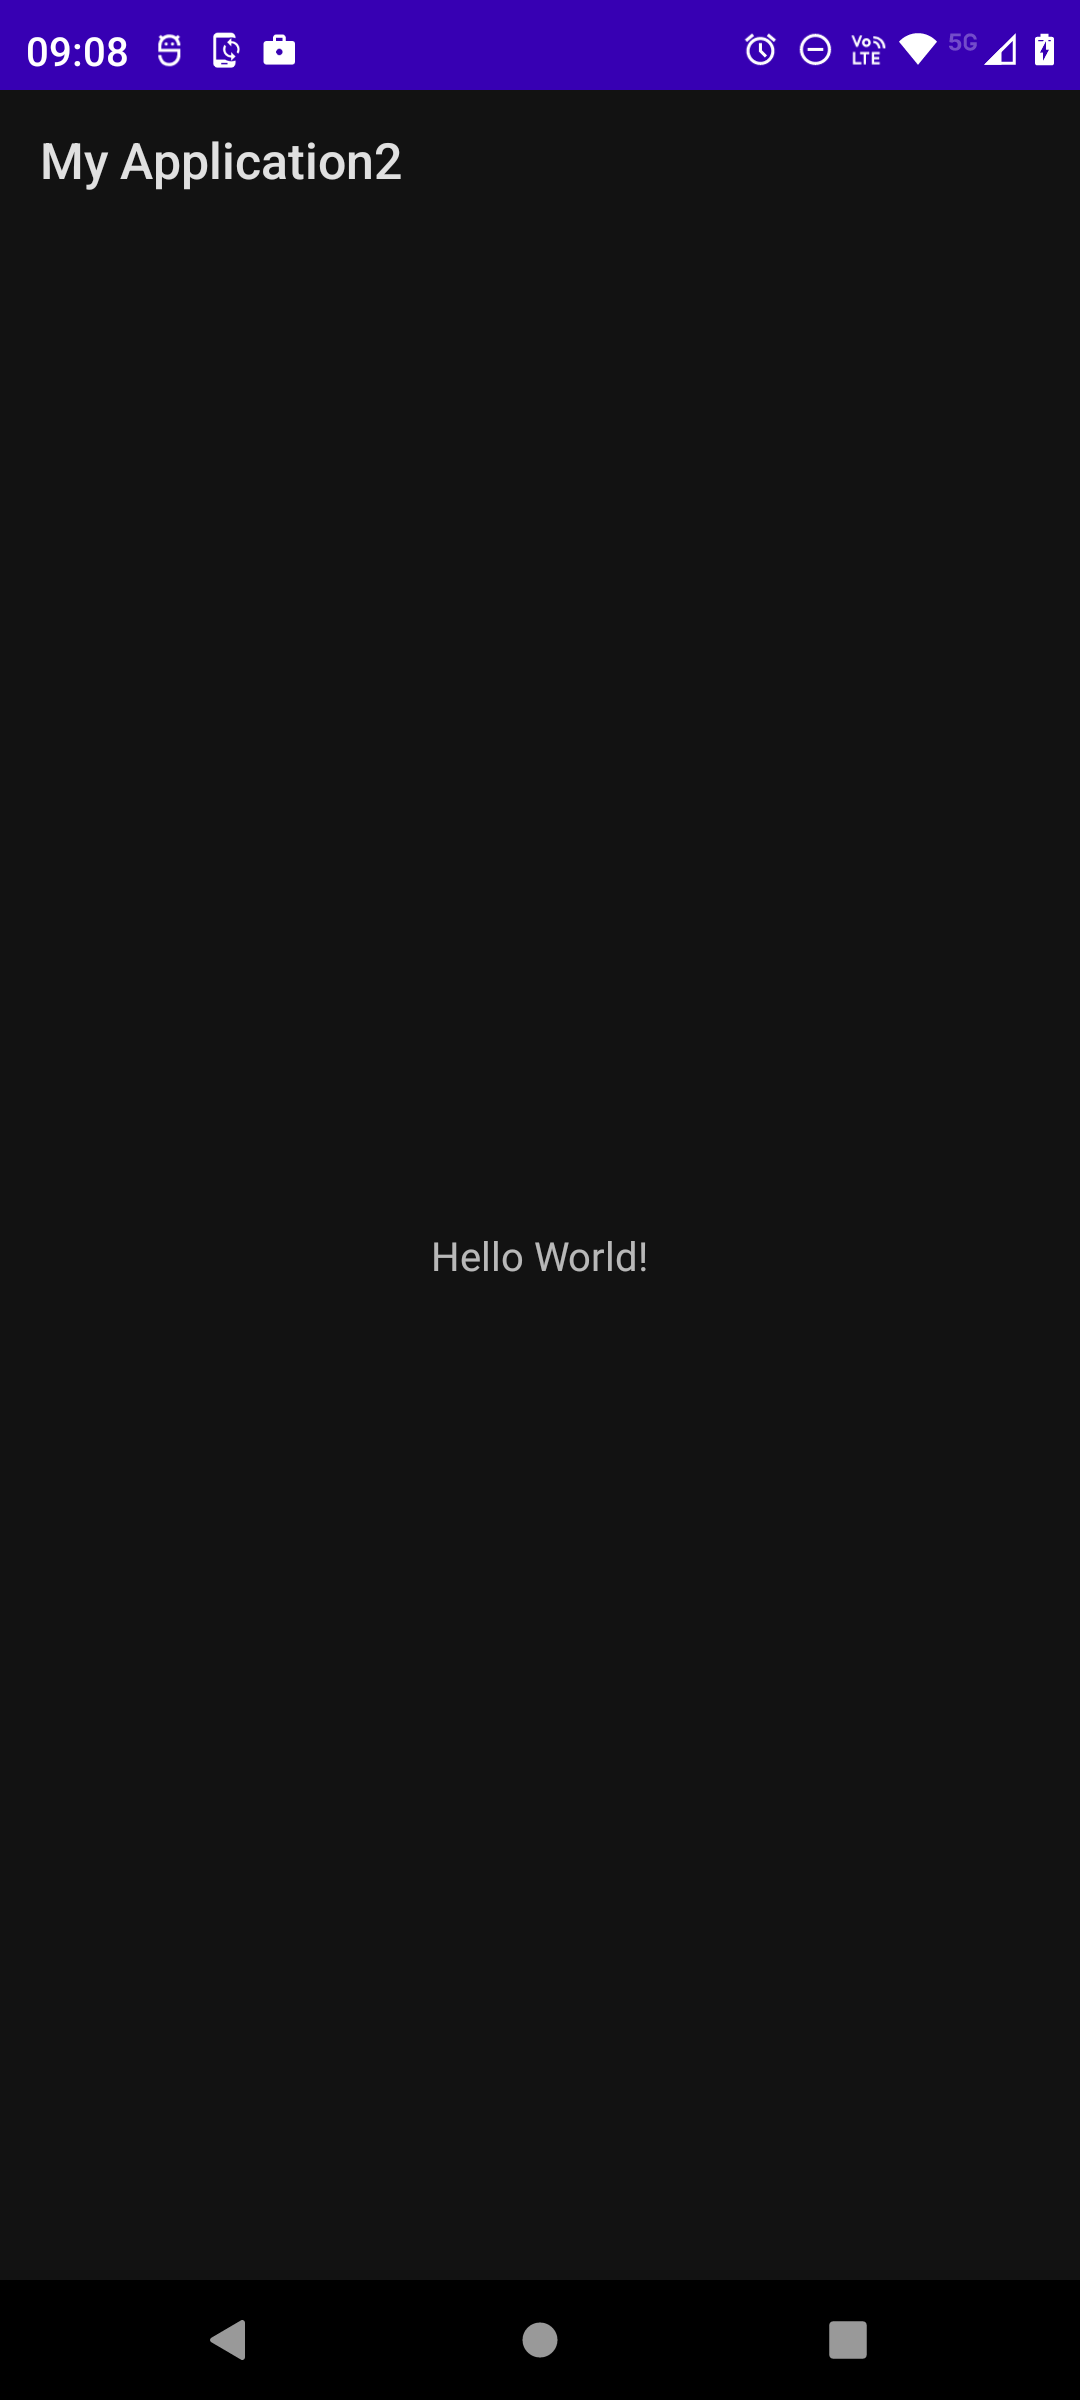
\includegraphics[width=0.95\linewidth]{01_Configurar/Etapa1_fase1.png}    
\end{center}
\end{columns} 
\end{frame}

